\section{Punto de Vista de Organización}

El punto de vista de la organización se centra en la organización (interna) de una empresa, un departamento, una red de empresas o de otra entidad organizativa. Es posible presentar modelos en este punto de vista como diagramas de bloques anidados, pero también de una manera más tradicional, como los organigramas. El punto de vista de la organización es muy útil para identificar las competencias, la autoridad y las responsabilidades de una organización.

\subsection{Modelo de Organización}
\begin{figure}[h!]
	\centering
	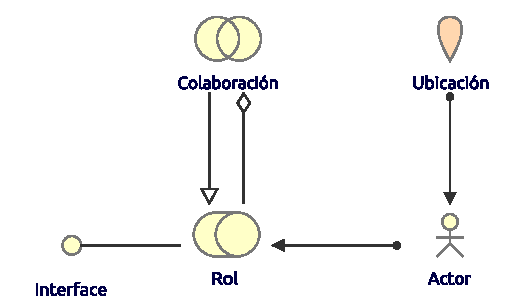
\includegraphics[width=.6\linewidth]{imgs/modelo/Organizacion}
	\caption{Modelo Organizacion}
\end{figure}

Un actor de negocios es una entidad de negocios que es capaz de realizar un comportamiento. Los actores pueden incluir entidades fuera de la organización real; por ejemplo, clientes y socios. Un actor comercial puede representar a esas entidades comerciales en diferentes niveles de detalle, y puede corresponder tanto a un actor como a una unidad organizativa en el marco del TOGAF. Ejemplos de actores comerciales son los seres humanos, los departamentos y las unidades comerciales. Una colaboración empresarial es un conjunto de dos o más elementos de la estructura activa interna de la empresa que trabajan juntos para llevar a cabo un comportamiento colectivo. Una interfaz de negocios es un punto de acceso en el que se pone a disposición del entorno un servicio comercial. Una interfaz comercial expone la funcionalidad de un servicio comercial a otros roles o actores comerciales. Se suele denominar canal (teléfono, Internet, oficina local, etc.). El mismo servicio comercial puede estar expuesto a través de diferentes interfaces.

\newpage
\subsection{Caso  de Organización}
\begin{figure}[h!]
	\centering
	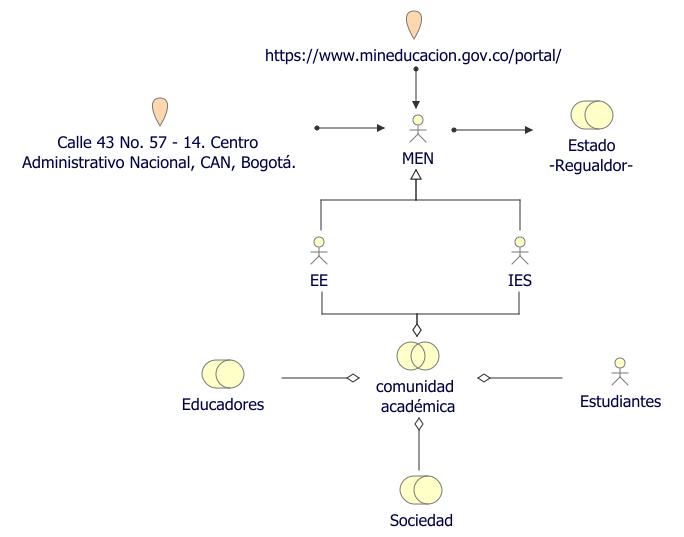
\includegraphics[width=.9\linewidth]{imgs/caso/negocio/organizacion}
	\caption{Caso Organizacion}
\end{figure}

El MEN tiene como actores principales los establecimientos educativos (EE), las instituciones de educación superior (IES) y las comunidades estudiantiles respectivas. Además, cuenta con ubicaciones tanto física como virtual, a saber, dispone de una dirección electrónica de dominio gubernamental como lo es \url{https://www.mineducacion.gov.co/portal/} y de una dirección física ubicada en la calle 43 No. 57 - 14 Centro 
Administrativo Nacional, CAN, Bogotá. Por otra parte, encontramos tres roles a destacar siendo el Estado uno de ellos y ejerciendo como ente regulador de las políticas a majear, así como, de emisor de recursos económicos junto con otro rol como lo es la sociedad y que, a su vez esta sociedad junto con el último de los roles a destacar, los educadores, colaboran o confluyen en una comunidad académica junto con los estudiantes, como otro de los actores principales de la organización.

